\chapter{Geoid problem}\label{chap:content}

Geoid, in the field of geodynamics, represents the shape of a gravity equipotential across the whole Earth's surface. Detailed maps of geoid elevation with contours spaced as close as 1 meter can show the effect of tectonic features such as deep sea trenches, outer arc rises, and oceanic ridges and troughs on the height of the geoid, which could provide powerful constraints that must be satisfied by the next generation of geodynamic models along with other data such as high quality determinations of surface deformation and new high resolution seismic data. \citep{10.1038_299104a0}

As shown in Figure \ref{figure:geoid_factors}, geoid is generally related to both the 3D density field of the Earth and the radial viscosity profile of the Earth's mantle. However, research shows that modelling that treats the geoid as being purely based on density variation near the surface can poorly explain the accurately observed geoid measurements with a satellite. \citep{10.1098_rsta.1989.0038}

Therefore, in this research, we aim to use Neural Networks as a way to forward model the geoid problem, assuming that viscosity varying in the radial direction with depth is the most important factor.

\begin{figure}[H]
    \centering
    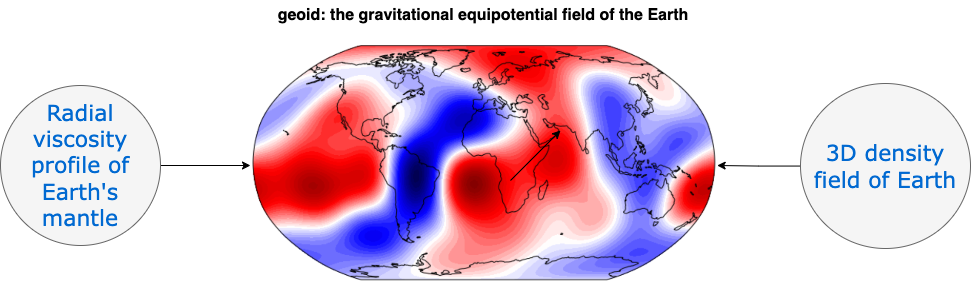
\includegraphics[scale=0.4]{figures/geoid_images/Geoid.png}
    \caption{Geoid and its two related factors.}
    \label{figure:geoid_factors}
\end{figure}

To explore the usage of Earth's viscosity to model the geoid using NNs, we use a 1D spherically symmetric viscosity model to compute a geoid surface in terms of some spherical harmonics coefficients that can be used to construct the geoid surface.\citep{10.1029_jb089ib07p05987} To further simplify this problem, the dataset used for this research uses a reduced prior such that the perturbations to the output are smaller.


\section{Dataset of geoid problem}

The reduced dataset consists of 1,000 pairs of input and output. In the dataset, the input is a vector with 257 values indicating a 1D spherically symmetric viscosity model and the output is a vector with 60 values representing a set of spherical harmonic coefficients describing the geoid height on the surface of the Earth. Figure \ref{figure:geoid_sample} shows a sample geoid field constructed from a random set of 60 geoid coefficients from the output data, where the units of the geoid are in metres and represent values greater or less than some reference value.

\begin{figure}[H]
    \caption{Sample geoid field.}
    \label{figure:geoid_sample}
    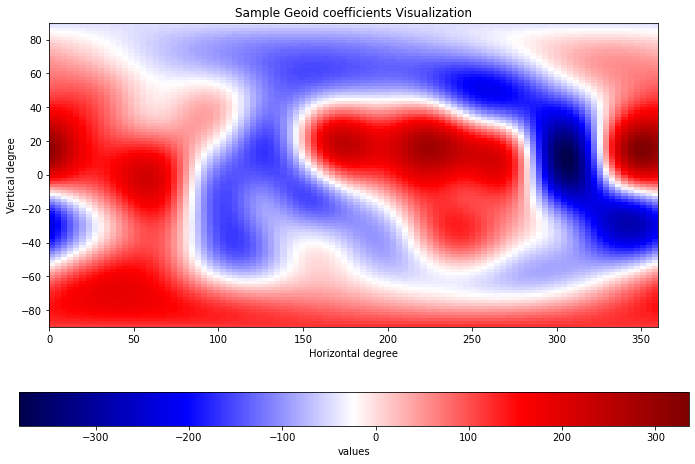
\includegraphics[scale=0.6]{figures/geoid_images/Geoid_Sample_visualization.png}
\end{figure}

To further observe the patterns in the input and output, 10 pairs of input and output are plotted in Figure \ref{figure:geoid_input} and Figure \ref{figure:geoid_output}, respectively.

\begin{figure}[H]
    \centering
    \caption{Every 100th input in the dataset.}
    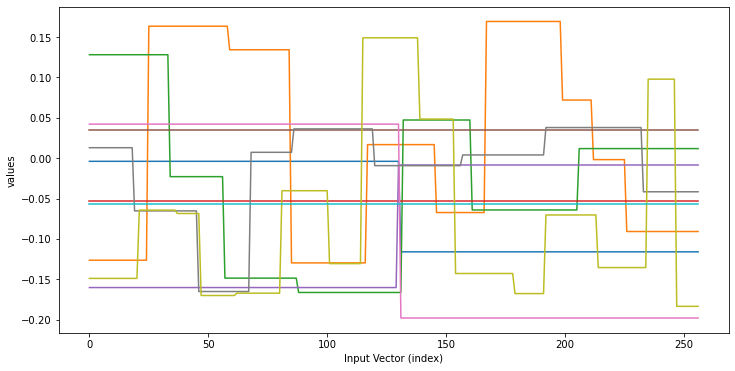
\includegraphics[scale=0.5]{figures/geoid_images/Geoid_sample_input.png}
    \label{figure:geoid_input}
\end{figure}

\begin{figure}[H]
    \centering
    \caption{Every 100th output in the dataset.}
    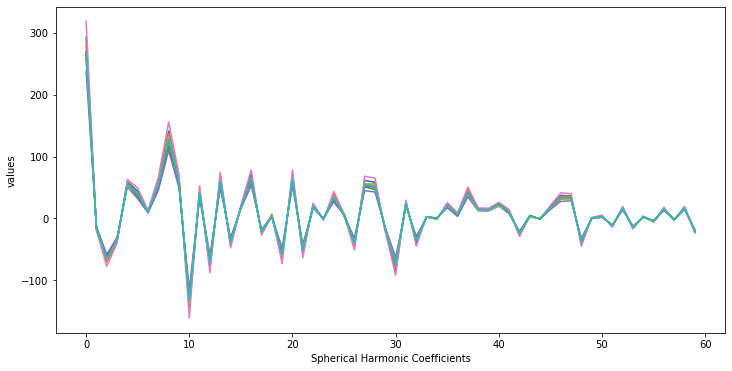
\includegraphics[scale=0.5]{figures/geoid_images/Geoid_sample_output.png}
    \label{figure:geoid_output}
\end{figure}

From Figure \ref{figure:geoid_output} we can observe that the outputs in the dataset can be seen as ``curves'' with the same pattern but with different amplitude. In this case, each of the 60 coefficients in the output data are normalised to be between 0 and 1 using their maximum and minimum values separately before feeding them into the neural network. This is because each of the parameters in an output vector can be seen as equally important and we want to prevent the neural network from spending most of its effort learning the parameters with a higher range of values. Hence, one can expect a higher accuracy when the parameters in the output data are standardized to the same range, which is supported by the evidence where we used data that is not normalized and got a lower accuracy.

After the output data is normalised, the entire dataset is randomly divided in a ratio of 8:1:1: 80 per cent of the dataset is used for training, 10 per cent for testing accuracy and the remaining 10 per cent to perform validation during training and prevent overfitting. For a dataset with 1,000 samples, this results in a train-test-validation split of 800-100-100.

\section{Fully Connected Neural Network for prediction}

To test the feed-forward fully connected neural network (FNN) with different configurations (e.g. different number of hidden layers and neurons per hidden layer) or other sets of hyperparameters (e.g. optimizer), a systematic testing method is applied. This method was implemented using three files: one text file to store all the different sets of FNN configurations and hyperparameters in a text format\footnote{Link to the file: \url{https://github.com/GiteonCaulfied/COMP4560_stokes_ml_project/blob/main/ModelList.txt}}, one Jupyter Notebook file to fetch all these combinations of configurations and hyperparameters line by line, build them as FNN models and train these models\footnote{Link to the file: \url{https://github.com/GiteonCaulfied/COMP4560_stokes_ml_project/blob/main/Geoid_systematic_training.ipynb}}, and another Jupyter Notebook for evaluation and visualisation of the trained models by specifying the path of a trained model.\footnote{Link to the file: \url{https://github.com/GiteonCaulfied/COMP4560_stokes_ml_project/blob/main/Geoid_visualisation.ipynb}}

The trained FNN architecture (in the format of a light-weight file) along with another text file contains the training loss and validation loss during training are stored in a specified path for further evaluation and visualisation. The name of these two files uniquely defines each experiment by including the values of hyperparameters used to generate this model in the file names. These files are also put in separate folders with the folder name associated with commit IDs to handle tracking of the process during the research in an educated or extensible way.

In this way, one can open the same Jupyter Notebook in different browser tabs, and then visualize simultaneously different models in different tabs using a cell in which the paths to the FNN model and its training data are specified. 

The systematic testing capability is implemented here to ensure traceability. In other words, as different values of the hyperparameters are tested, we wanted to be able to record the results (e.g., the trained network and the training data) so that we do not have to repeat them again or rely on our memory to compare the performance of different configurations.

Also, to prevent overfitting, a variation of the early-stopping method is used during training. The normal early-stopping method lets the network train until the error function evaluated on the validation set starts to increase beyond a certain threshold \citep{10.1007_978-3-642-35289-8_5}, while the variant used here just stores the best model during training (the one with the lowest validation loss) in a specified path and allows the network to keep training as normal. In this case, the output model is the best model instead of the trained model at the last optimization iteration. This method is also used in the upcoming chapters with the ConvAE, FNN and LSTM networks to solve the 2D mantle convection problem.

After testing with NNs with different number of hidden layers and neurons per hidden layer, we found that FNNs with a total number 3-4 hidden layers performed the best.

In the following figures, we present results from a FNN with 4 hidden layers with 200, 160, 120 and 80 neurons in each layer, respectively, ReLU as activation function, mean squared error (MSE) as loss function, and trained for 200 epochs using Mini-Batch Gradient Descent (with a batch size of 16).

Note that the loss value (error), which is back-propagated during the training process, is defined as the MSE between the prediction and the normalised ground truth. In this case, the best and worst cases shown below are also defined upon the value of this normalised loss, instead of the reconstructed loss which is defined as the MSE between the inverse normalised prediction and the ground truth.

We present the training loss and validation loss in Figure \ref{figure:geoid_losses} and the overall testing result in Figure \ref{figure:geoid_testing}.

\begin{figure}[H]
    \caption{Training and validation loss.}
    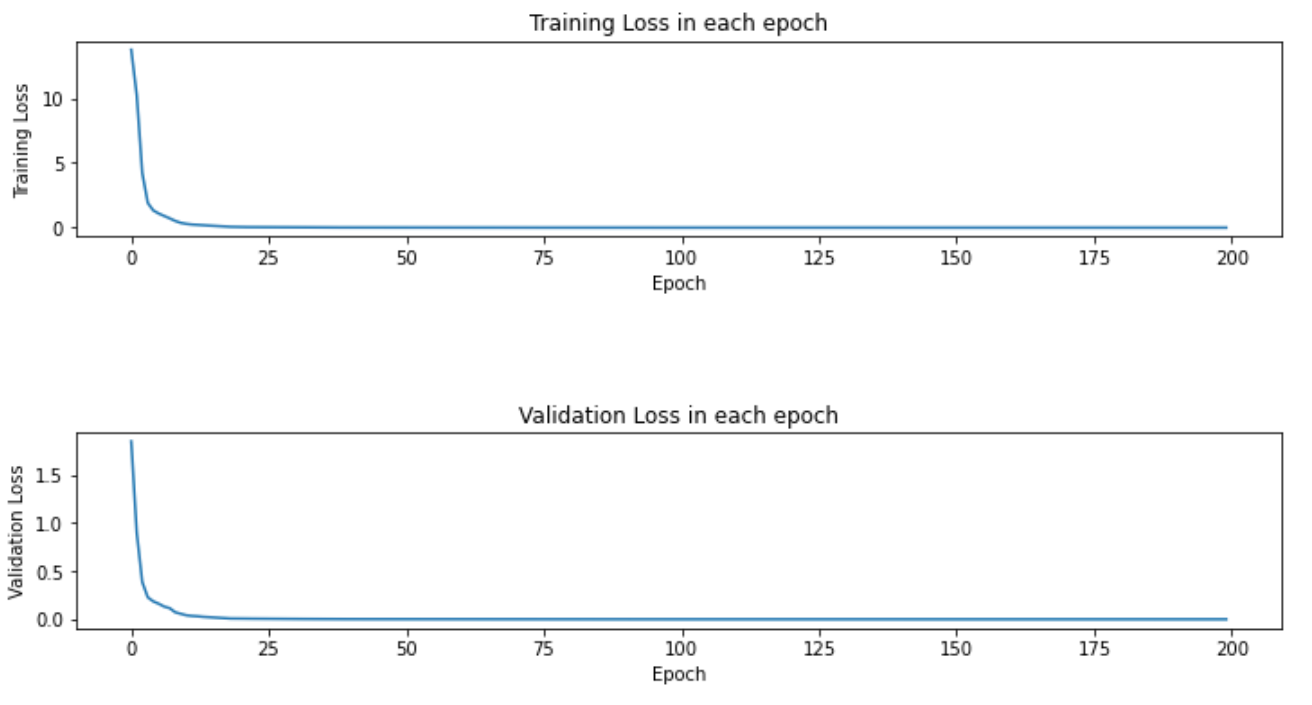
\includegraphics[scale=0.6]{figures/geoid_images/Geoid_trainingData.png}
    \label{figure:geoid_losses}
\end{figure}

\begin{figure}[H]
    \caption{Overall testing result. If the normalised loss for a prediction is less than the threshold, then the prediction is considered to be accurate. Multiple thresholds are set to evaluate the general performance by comparing these threshold with the normalised error shown in best and worst cases.}
    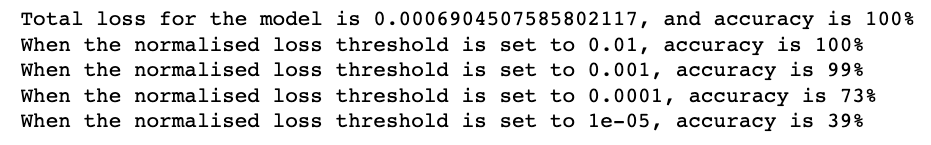
\includegraphics[scale=0.8]{figures/geoid_images/Geoid_OverallTesting.png}
    \label{figure:geoid_testing}
\end{figure}

The most accurate geoid prediction and the least accurate geoid prediction are presented in Figure \ref{figure:geoid_best} and Figure \ref{figure:geoid_worst}, respectively.

\begin{figure}[H]
    \caption{Most accurate geoid prediction, including the input viscosity model resulting in this prediction, the ground truth and the prediction in the same plot, and the error plot calculated as the difference between the prediction and the ground truth.}
    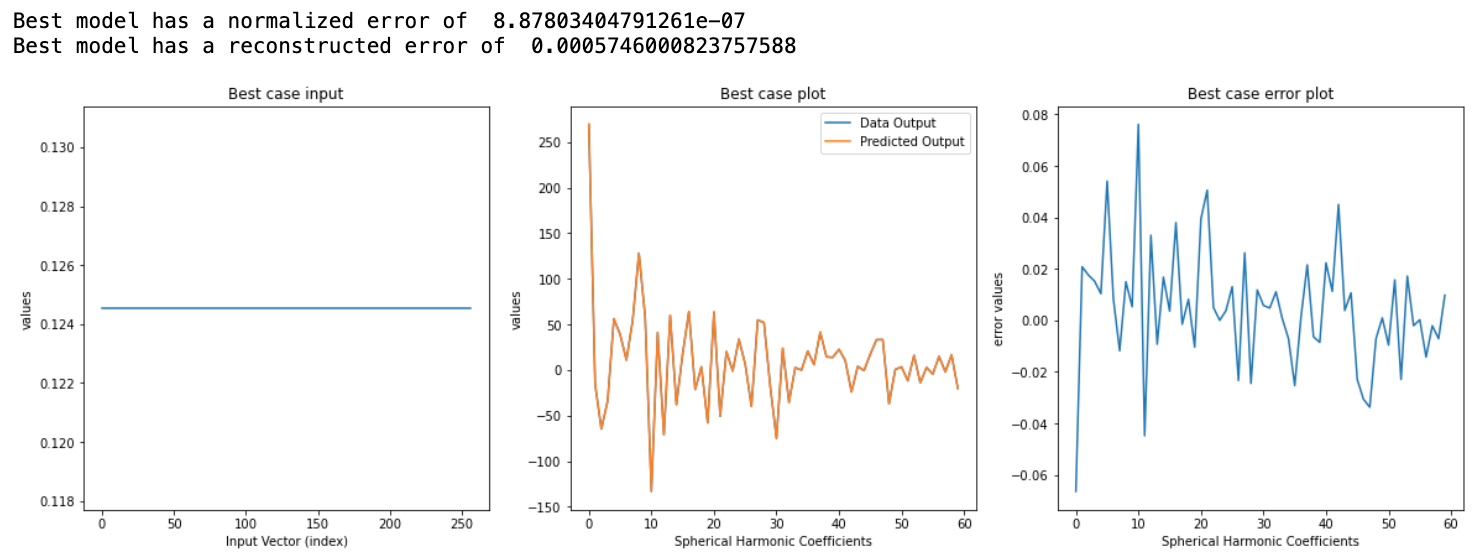
\includegraphics[scale=0.6]{figures/geoid_images/Geoid_Best.png}
    \label{figure:geoid_best}
\end{figure}

\begin{figure}[H]
    \caption{Least accurate geoid prediction, including the input viscosity model resulting in this prediction, the ground truth and the prediction in the same plot, and the error plot calculated as the difference between the prediction and the ground truth.}
    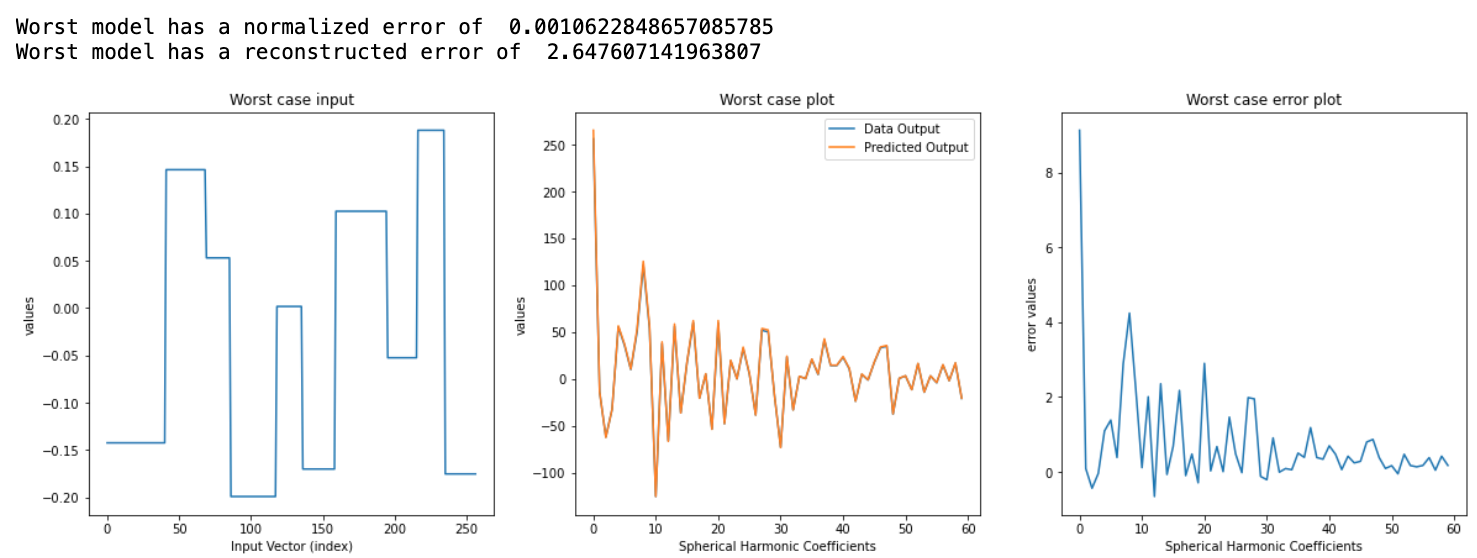
\includegraphics[scale=0.6]{figures/geoid_images/Geoid_Worst.png}
    \label{figure:geoid_worst}
\end{figure}

On average, both the normalised loss and the reconstructed loss are low and no overfitting occurs. The accuracy of the prediction is nearly 100\% when the threshold is set to be 10 times lower than the worst loss value. 

In order to provide further evidence, the geoid fields constructed using the set of 60 coefficients produced by the FNN in both the best case and the worst case are visualized in Figure \ref{figure:geoid_best_visual} and Figure \ref{figure:geoid_worst_visual}, along with the fields produced by the ground truth and the error maps representing the difference between the prediction and the ground truth.

\begin{figure}[H]
    \caption{Visualization of the most accurate geoid prediction.}
    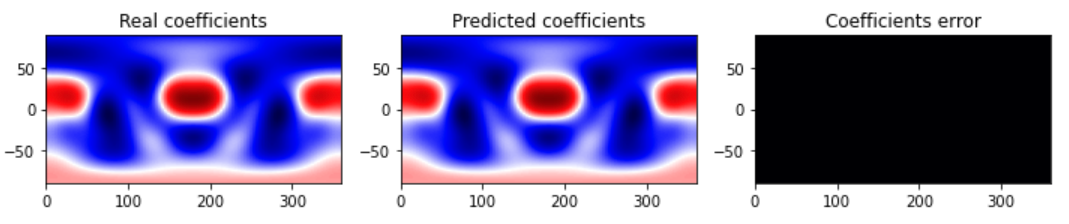
\includegraphics[scale=0.4]{figures/geoid_images/Geoid_Best_visualization.png}
    \label{figure:geoid_best_visual}
\end{figure}

\begin{figure}[H]
    \caption{Visualization of the least accurate geoid prediction.}
    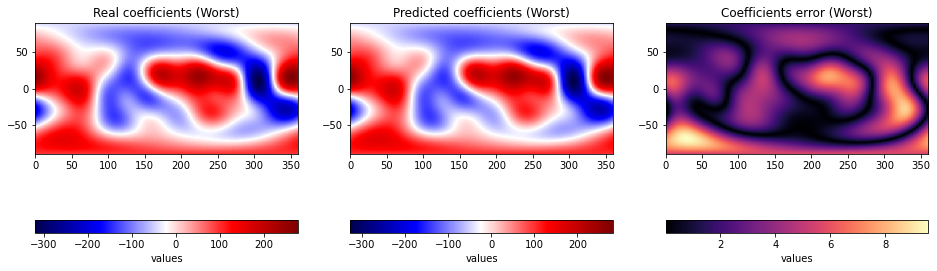
\includegraphics[scale=0.4]{figures/geoid_images/Geoid_Worst_visualization.png}
    \label{figure:geoid_worst_visual}
\end{figure}

We can observe that the result produced by the FNN is in high agreement even in the worst case, where the maximum error between the real geoid field and the predicted geoid field is about 60 times less than the range of real values. The real geoid field and the predicted field also have the same patterns in both cases, meaning that FNN is able to capture the main features of the data in its prediction.

Overall, we constructed a systematic framework for rapidly testing different FNN architectures in a reproducible way, and we were able to create a highly accurate FNN as a surrogate forward model for the geoid problem. This represents a first remarkable milestone for further research in inverse problems involving observations of the Earth's geoid.